%-------------------------------------------------------------------------------
%                            BAB III
%               		METODOLOGI PENELITIAN
%-------------------------------------------------------------------------------
% \fancyhf{} 
% \fancyfoot[R]{\thepage}
\chapter{METODE PENENILITIAN}
%\thispagestyle{plain} % Halaman pertama bab menggunakan gaya plain
\section{Waktu dan Lokasi Penelitian}
Penelitian ini akan bertempat pada beberapa ruangan yang digunakan oleh mahasiswa Jurusan Informatika USK yang umumnya terletak pada lantai 3 blok A dan blok E Gedung Fakultas MIPA USK. Waktu yang dibutuhkan agar penelitian ini dapat di implementasikan adalah 4 bulan terhitung dari bulan Januari 2024 hingga Mei 2024.

\section{Alat dan Bahan}
Alat dan Bahan yang akan digunakan pada penelitian ini terdiri dari beberapa perangkat keras (\textit{hardware}) dan perangkat lunak (\textit{software}) yang dijabarkan sebagai berikut:

\begin{enumerate}
\item Perangkat Keras
	\begin{itemize}
	\item Laptop Apple Macbook Air M1 2020 dengan RAM 8 \textit{Gigabyte}.
    \end{itemize}
\item Perangkat Lunak
	\begin{itemize}
	\item MacOS (18.1)
	\item Jupyter 
	\item Python 3.8.17
    \item NumPy (1.24.0)
    \item SQLite3 (3.39.4)
    \item Pandas (1.5.3)
    \item Joblib (1.2.0)
    \item scikit-learn (1.2.0)
    \item TensorFlow (2.11.0)
    \item Keras (2.11.0)
    \item Matplotlib (3.6.2)
    \item TensorFlow Keras Layers (2.11.0)
    \item itertools (built-in)
	\end{itemize}
\end{enumerate}
\newpage
\section{Metode Penelitian}
\par Dalam pengembangan model Long Short-Term Memory (LSTM), persiapan data yang tepat adalah langkah krusial yang dapat mempengaruhi kinerja model secara signifikan. Bab ini membahas berbagai teknik untuk mempersiapkan data numerik dan kategorikal, serta bagaimana menangani urutan dengan panjang yang bervariasi.
\par Gambar \ref{fig:lstm_architecture} menunjukkan arsitektur dasar dari LSTM. Dalam arsitektur ini, terdapat tiga komponen utama: input layer, hidden LSTM layer, dan output layer.

\begin{figure}[h]
    \centering
    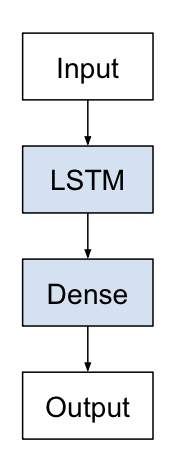
\includegraphics[width=0.2\textwidth]{image/lstm1.png} 
    \caption{ LSTM Data kategorikal perlu diubah menjadi format numerik agar dapat digunakan dalam model LSTM. Dua metode umum untuk melakukan ini adalah One-Hot Encoding dan Label Encoding. One-Hot Encoding mengubah setiap kategori menjadi vektor biner, sedangkan Label Encoding memberikan setiap kategori nilai integer \citep{brownlee2017}}
    \label{fig:lstm_architecture}
\end{figure}
\section{Persiapan Data Numerik}
\par Data numerik memerlukan normalisasi atau standardisasi sebelum digunakan dalam model LSTM. Normalisasi membantu dalam mengurangi skala data, sehingga mempercepat proses pelatihan dan meningkatkan konvergensi model. Metode umum yang digunakan termasuk Min-Max Scaling dan Z-score Normalization \citep{brownlee2017}.

\subsection{Normalisasi}
\par Normalisasi data dilakukan dengan rumus:
$$
I' = \frac{I - I_{min}}{I_{max} - I_{min}}
$$
di mana $$I'$$ adalah data yang dinormalisasi, $$I$$ adalah data asli, $$I_{min}$$ dan $$I_{max}$$ adalah nilai minimum dan maksimum dari dataset.

\section{Persiapan Data Kategorikal}
\par Data kategorikal perlu diubah menjadi format numerik agar dapat digunakan dalam model LSTM. Dua metode umum untuk melakukan ini adalah One-Hot Encoding dan Label Encoding. One-Hot Encoding mengubah setiap kategori menjadi vektor biner, sedangkan Label Encoding memberikan setiap kategori nilai integer \citep{brownlee2017}.

\subsection{One-Hot Encoding}
\par One-Hot Encoding dapat dilakukan dengan menggunakan pustaka seperti scikit-learn. Misalnya, untuk mengubah kolom kategorikal menjadi format one-hot:
\begin{verbatim}
from sklearn.preprocessing import OneHotEncoder
encoder = OneHotEncoder()
encoded_data = encoder.fit_transform(data).toarray()
\end{verbatim}

\section{Menangani Urutan dengan Panjang Bervariasi}
\par Dalam banyak kasus, urutan data yang digunakan dalam LSTM memiliki panjang yang bervariasi. Untuk menangani ini, kita dapat menggunakan padding untuk menambahkan nilai nol ke urutan yang lebih pendek, sehingga semua urutan memiliki panjang yang sama. Keras menyediakan fungsi \texttt{pad\_sequences()} untuk tujuan ini.

\subsection{Padding}
\par Padding dapat dilakukan sebagai berikut:
\begin{verbatim}
from keras.preprocessing.sequence import pad_sequences
padded_sequences = pad_sequences(sequences, maxlen=max_length)
\end{verbatim}

\section{Prediksi Urutan sebagai Pembelajaran Terawasi}
\par Dalam konteks LSTM, prediksi urutan dapat dipandang sebagai masalah pembelajaran terawasi. Ini melibatkan transformasi data urutan menjadi format yang dapat digunakan untuk pelatihan model, di mana input dan output ditentukan berdasarkan langkah waktu tertentu \citep{brownlee2017}.


\par Persiapan data yang tepat adalah langkah penting dalam pengembangan model LSTM. Dengan menggunakan teknik yang tepat untuk normalisasi, encoding, dan padding, kita dapat meningkatkan kinerja model dan memastikan bahwa data siap untuk analisis lebih lanjut.

\begin{equation}
    \frac{n_i \cdot n_e}{n_a} = \left( \frac{2}{\Lambda^3} \right) \cdot \left( \frac{g_i}{g_a} \right) \cdot \exp \left( -\frac{E_{ion}}{kT} \right)
    \label{eq:rate}
\end{equation}


----------------------------------------------------------%
\begin{lstlisting}[language=Python, caption=Contoh Fungsi Python]
    def fibonacci(n):
        """Menghitung deret Fibonacci"""
        a, b = 0, 1
        for _ in range(n):
            print(a, end=' ')
            a, b = b, a + b
        return a
    \end{lstlisting}
----------------------------------------------------------
% Tanpa figure
\lstinputlisting[
    language=Python,
    caption= Ini adalah sebuah teorema.
    Ini adalah sebuah teorema.
    Ini adalah sebuah teorema.
    Ini adalah sebuah teorema.
    Implementasi Algoritma Dijkstra,
    label=code:dijkstra
]{/Users/birrulwalidain/skripsi-2/!project/src/train.py}



\begin{theorem}
Ini adalah sebuah teorema.
\end{theorem}

\begin{definition}
Ini adalah definisi.
\end{definition}

\begin{remark}
Ini adalah catatan tanpa nomor.
\end{remark} 

\begin{proof}
Ini adalah bukti.
\end{proof}
 \begin{example}
        f
 \end{example}


 \begin{table}[H]
    \centering
    \caption{Perbandingan Performa Model Performa Model Performa Model Performa Model Machine Learning pada Data LIBS}
    \label{tab:performa_ml}
    \centering
    \begin{tabular}{lcccc}
      \toprule
      Model & Akurasi (\%) & Presisi (\%) & Recall (\%) & RMSE \\
      \midrule
      Random Forest & 95.2 & 94.8 & 95.1 & 0.12 \\
      SVM & 89.7 & 88.5 & 90.2 & 0.21 \\
      Transformer & 97.1 & 96.9 & 97.0 & 0.08 \\
      CNN & 93.4 & 92.7 & 93.5 & 0.15 \\
      \bottomrule
    \end{tabular}
    
    \smallskip
    \footnotesize
    \textit{Keterangan:} Data diperoleh dari 100 sampel logam dengan 5 kelas komposisi.
  \end{table}


% Baris ini digunakan untuk membantu dalam melakukan sitasi
% Karena diapit dengan comment, maka baris ini akan diabaikan
% oleh compiler LaTeX.
%\begin{comment}
%\bibliography{daftar-pustaka}
%\end{comment}